\documentclass[../main.tex]{subfiles}
\usepackage[english]{babel}

\graphicspath{{\subfix{../images}}}
\begin{document}


\section{Datasets}
Two datasets composed by light-reflected images  were used in this work: 
\begin{itemize}
    \item \textit{Deepskin} dataset consists in 1564 human wound images obtained during routine dermatological exams in the Dermatology Unit at IRCCS Sant’Orsola-Malpighi University Hospital of Bologna;
    \item \textbf{Petwound} dataset is set of wound photos of dogs and cats acquired  at the University Veterinary Hospital of the Department of Veterinary Medical Sciences, University of Bologna.
\end{itemize}
Different trained clinicians had taken pictures with digital cameras during clinical practice.
For the image acquisition rigid or standardized protocols were not used during the procedure: for this reason, we can classify the entire set of data as natural images, with uncontrolled illumination, background, and exposition.
The images were acquired in proximity to the anatomical region of interest, trying to put the entire wound area at the center of the picture. 
The images were acquired according to the best judgment by each clinician with different devices and without using flash.
\subsection{Deepskin}
The analyzed images had been obtained during routine dermatological exams in the Dermatology Unit at IRCCS Sant’Orsola-Malpighi University Hospital of Bologna. 
We collected 474 patients over 2 years (from March 2019 to September 2021) at the center with a total of 1564 wound images (Deepskin dataset).
In Table \ref{tab:patients-deepskin} are showed the patients divided for sex, with their age range.

\begin{table}[!ht]
    \centering
    \begin{tabular}{c|c|c|c|}
    
         & \textbf{Male} & \textbf{Female} & \textbf{Tot} \\ \hline
        \textbf{N° patients} & 210 & 264 & 474 \\ 
        \textbf{Age} & 71 ± 17 & 77 ± 17 & 74 ± 20 \\ \hline
    \end{tabular}
    \caption{Description of the patient population involved in the study. The number of patients is split according to sex and age.}
    \label{tab:patients-deepskin}
\end{table}
The dataset collection was performed during clinical routine, therefore chronic patients are included in the study.
For this reason, there are different pictures of the same wound acquired at different time points. 
Moreover, an heterogeneous population was selected for the dataset composition, thus the dataset includes samples with ulcers at different healing stages and in different anatomical positions.
The Table \ref{tab:wounds-deepsk} represents the number of samples for each anatomical position as well as the number of wounds for the same region.

\begin{table}[!ht]
    \centering
    \begin{tabular}{c|c|c|c|c|c|}
  
        \textbf{} & \textbf{Foot} & \textbf{Leg} & \textbf{Chest} & \textbf{Arm} & \textbf{Head} \\ \hline
        \textbf{N° wounds} & 97 & 354 & 14 & 6 & 2 \\ 
        \textbf{N° images} & 364 & 1142 & 38 & 13 & 7 \\ \hline
    \end{tabular}
    \caption{Description of the images involved in the study. The number of images is split according to anatomical positions. The same wound could have been acquired at different time points: we report in the last row the number of images associated to each anatomical position.}
    \label{tab:wounds-deepsk}
\end{table}
A Smartphone digital camera (Dual Sony IMX 286 12MP sensors with 1.25µm pixel size, 27mm equivalent focal length, F2.2 aperture, Laser-assisted AF, DNG Raw capture) acquired the raw images under uncontrolled illumination conditions, various backgrounds, and image expositions for clinical usage.

\subsubsection{Data annotation}
145 randomly chosen images were manually segmented by two expert clinicians.
The annotation was performed by the first expert and reviewed by the second one to improve the data reliability.
The masks, annotated by the experts, consisted in binary images where the wound area is highlighted with respect to the background.
This set of images-masks was used as ground truth for our deep learning model. 
A pixel-wise annotation is hard to obtain also for expert clinicians and particularly time consuming.
For this reason, we have chosen to minimize the number of manual annotations.
This small core set of manual annotations was used as a kick starter for an active semi-supervised training procedure via deep learning segmentation model. 
The initial set of segmentation masks was relatively rough, mostly consisting of polygonal shapes. 


\subsection{Petwound}
A set of wound photos of dogs and cats was acquired with 4 different digital cameras at the University Veterinary Hospital of the Department of Veterinary Medical Sciences, University of Bologna, during daily clinical practice.
The acquisition procedure was performed from April 2014 to June 2022, with a total of 290 selected images (Petwound dataset). 
The photo included spontaneous wounds of owned dogs and cats that were brought to the institution for the treatment of the wound and eventually other concomitant lesions.
To be enrolled in the study images must contain a cutaneous region with an open wound caused by cuts, abrasions, laceration, sores, burns, degloving injuries, avulsion wound, or dehiscence from previous surgery.
Althought the total images producted by clinicians were 406, exclusion criteria were set from both a technical and a clinical point of view:
\begin{itemize}
    \item rejection because of poor quality: some images showed no sharp definition, inadequate light exposition;
    \item rejection of non proper wounds: kind of injuries represented could not be categorized as spontaneous wounds (open wound during surgery, sutured wounds, and wounds with other surgical implants); 
    \item rejection because of background: images with bloodstains or red-colored objects in the background were also excluded only in extreme cases. 
    Many images with various backgrounds have been included in the dataset to strengthen the generalization capability of the trained models.
\end{itemize} 
The total count of initial and included images, as well as the statistics of species involved are reported in Table \ref{tab:PetWound}. 
As for Deepskin, the presence of an higher number of included images with respect to wounds indicates that some wound images depict the same injury at different times.
\begin{table}[!ht]
    \centering
    \begin{tabular}{c|c|c|c|}

        \textbf{} & \textbf{Dog} & \textbf{Cat} & \textbf{Tot } \\ \hline
        \textbf{N° initial images} & 301 & 105 & 406  \\ 
        \textbf{N° included images} & 208 & 82 & 290  \\ 
        \textbf{N° included wounds} & 130 & 47 & 177  \\ \hline
    \end{tabular}
    \caption{Description of the images involved in the study. The number of images is split according to the animal species of the patients. The three rows of the table show: the number of initial images collected; the number of images after exclusion of inadequate ones; the different wounds considered starting from the included images, since the same wound could have been acquired at different time points in dogs and cats.}
    \label{tab:PetWound}
\end{table}
The images were acquired during clinical practice by several operators without a standardized procedure. 
The aim was to obtain an heterogenous dataset, with different light conditions (illumination and exposition) and variable backgrounds.
All the images were stored as RGB 8-bit JPEG format with different dimensions according to the device used. The details of the camera devices used for the acquisition are showed in Table \ref{tab:device-PetWound}.

\begin{table}[!ht]
    \centering
    \scalebox{0.7}{     \begin{tabular}{c|c|c|c|c|}
    
        \textbf{} & \textbf{Redmi Note 9 Pro } & \textbf{Redmi Note 5} & \textbf{ASUS Z017D} & \textbf{Olympus Imaging CORP } \\ \hline
        \textbf{F-stop } & f/1.9  & f/1.9  & f/2  & f/3.5 \\ 
        \textbf{Exposition } & 1/33 sec  & 1/25 sec  & 1/100 sec  & 1/15 sec \\ 
        \textbf{Iso sensibility } & ISO-330  & ISO-200  & ISO 71  & ISO-71 \\ 
        \textbf{Focal distance } & 5 mm  & 4 mm  & 4 mm  & 4 mm  \\ 
        \textbf{Focal length } & 25 mm  & 24 mm  & not specified  & not specified \\ \hline
    \end{tabular}
    }
    \caption{Main specifics of the camera devices used for the acquisition of the photos. The Petwound database is composed by images acquired with three different camera devices. In details, there are three different smartphone digital cameras and an Olympus digital camera.}
    \label{tab:device-PetWound}
\end{table}

\section{Models}

In this work we chose a deep CNN U-Net with two architectures: an EfficientNet-b3 \cite{tan2019efficientnet} and a MobileNet-v2 \cite{sandler2018mobilenetv2} backbone for the automated segmentation.
The EfficientNet-b3 represents the state of the art considering the ratio between accuracy and number of parameters. 
After several trials  with different CNN architectures, it was chosen to be the best model able to balance our needs.
On the other hand the MobileNet-v2, with its lower number of parameters, represents the suitable model for possible mobile implementations. 
The difference in terms of parameters between the two specifications is highlighted in Table \ref{tab:models-parameters}.

\begin{table}[H]
    \centering
    \begin{tabular}{l|l|l|}
    
         Loss & EfficientNet-b3 & MobileNet-v2 \\ \hline
        Non-trainable parameters & 89,280 & 36,096 \\ \hline
        Trainable parameters & 17,778,553 & 8,011,345 \\ \hline
        Total parameters & 17,867,833 & 8,047,441 \\ \hline
    \end{tabular}
    \caption{Number of model parameters for EfficientNet and MobileNet specifications.  MobileNet results having half of parameters with respect to EfficientNet.}
    \label{tab:models-parameters}
\end{table}

\section{Training strategy}
Two different training strategies were adopted for Deepskin and Petwound datasets. 
Both of them are based on the ASSL procedure of Figure \ref{fig:ASSL} to deal with the problem of annotation availability, while minimizing the effort for clinicians. 
This procedure works by training the model on the labelled image iteratively.
Since only a small fraction of Deepskin images were provided with a ground truth, the segmentations generated by the model were submitted to the two expert clinicians. 
At each round, for each validation image, the clinicians determined if the generated segmentation was accurate according to the following binary criteria:
\begin{itemize}
    \item  the mask covers the entire wound area;
    \item the mask covers only the wound area, i.e. the mask must not have holes or spurious parts;
    \item the mask shape follows the correct wound boundaries.
\end{itemize}
The validation images and corresponding segmentation masks with all the criteria were inserted into the training set for the next round of model training.


\begin{figure}[H] 
\begin{center}
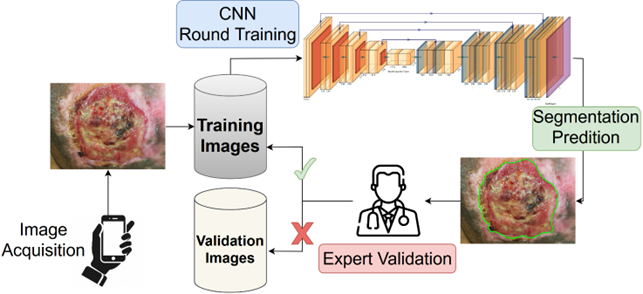
\includegraphics[width=16cm]{images/ASSL.png}
\caption{\small{Representation of the active semi-supervised learning strategy implemented for the training of the wound segmentation model.}}\label{fig:ASSL}
\end{center}
\end{figure}

Slightly different strategies were developed for Deepskin and Petwound because of the different number of manually annotated images of the datasets: 145 for Deepskin, 0 for Petwound.

\subsection{Deepskin}

For the EfficientNet architecture, we used 145 manually annotated images as starting point for the ASSL pipeline.
After each training, clinicians repeated the evaluation of automated segmentations until the number of training data reached (at least) the 80\% of available samples.
To quantify the generallization capability of the model, we divided the available image-masks samples into training - test sets (90\% - 10\%) for each round of training.
Moreover, we quantified the percentage of images correctly segmented on the validation according to the clinicians evaluation.

The correctly annotated images after the ASSL training of EfficientNet were used to train a MobileNet-v2 model  to check its capability to segment such images with a lower number of parameters.

Both trained models were used for the TL procedure to be able to segment automatically wound images belonging to Petwound dataset.

\subsection{Petwound}

Appling the principles of Transductive TL, we aimed to transfer knowledge from Deepskin to Petwound, since the type of data of the two datasets could be considered belonging to similar domains.

We used the EfficientNet model trained on the human wound Deepskin dataset without any refinements to produce the initial labels for the pet wound images. 
This procedure substitutes the manual annotation for the initial round of the ASSL pipeline used in Deepskin training.
At each round of ASSL, the model weights were restored to the original configuration obtained by the training on the Deepskin dataset, i.e. a human-based wound dataset.
The full procedure is showed in Figure \ref{fig:TASSL}.
The use of a pre-trained configuration of the model weights during ASSL rounds facilitates the learning process, providing a solid starting point for a TL procedure. 

\begin{figure}[H] 
\begin{center}
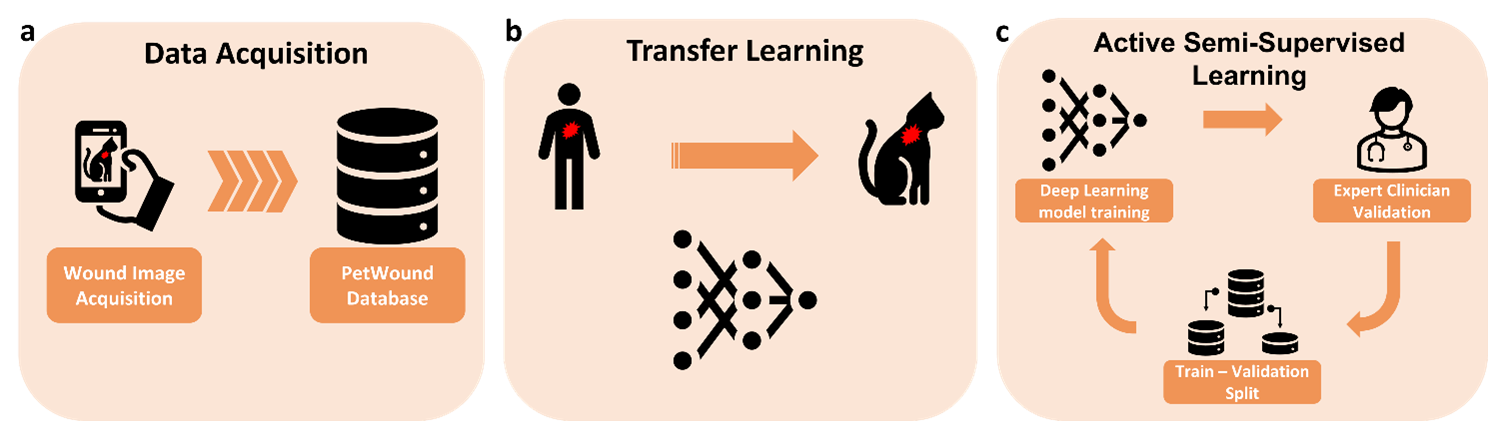
\includegraphics[width=16cm]{images/TASSL.png}
\caption{\small{Representation of the pipeline implemented for the training of the EfficientNet model.
a) The images acquired during clinical practice are used as data for the ASSL procedure.
b) At the first round the initial set of labelled images was obtained by the application of the model pre-trained on the Deepskin dataset, without any refinement of the model parameters.
c) The obtained set of labelled images was used as the kick-start for the ASSL training strategy, performing a TL from the human-based wounds to the pet ones. 
At each round of training the model was reset to the initial conditions, i.e. the parameters obtained by the training on the Deepskin dataset.}}\label{fig:TASSL}
\end{center}
\end{figure}
An analogous pipeline of ASSL in combination with TL was used for the training of a MobileNet U-Net architecture. 
The MobileNet model, previously trained on Deepskin, was used in the ASSL training strategy as described for the EfficientNet one. 
The implementation of the ASSL training strategy aims to increase progressively the number of correctly annotated samples.
Starting from a small fraction  of the original set of data, labelled with the application of TL, we aimed to reach at least the 80\% of correct segmentations. 
At each round of ASSL, we split randomly the labelled data into two disjoint sets of images, using the 90\% of the images for the training and the 10\% for the performance evaluation.



\section{Metrics}

The efficiency of the ASSL training was evaluated according to the number of correctly segmented images after clinical evaluation.
Additionally, in order to prevent possible overfitting of the model during the training stage, we monitored the efficiency of the model using standard metrics.
The number of correct segmentations was evaluated on the total datasets, while the efficiency metrics were quantified on the 10\% of images used for the performance evaluation.
In the following subsections, the metrics chosen for each training are reported.

\subsection{Deepskin}


The EfficientNet model trained on deepskin dataset was evaluated with Precision, Recall and Dice coefficient:

\begin{equation}\label{eq:precision}
    Precision=\frac{TP}{TP+FP}
\end{equation}

\begin{equation}\label{eq:recall}
    Recall=\frac{TP}{TP+FN}
\end{equation}

\begin{equation}\label{eq:dsc}
    DSC=\frac{2\ \times T\ P}{2\times T\ P+FN+FP}
\end{equation}
where TP, FP, and FN are the True Positive, False Positives, and False Negative scores.
Precision metric is able to evaluate the fraction of true instances among all the predicted one, whereas Recall describes the fraction of true predictions with respect to the total ones that should be detected. DSC measures the similarity between the detected ground truth and all the detected instances.

For the MobileNet training, the metrics evaluated were $F_{1}$ and IoU scores.
Starting from the definition of Precision (Equation \ref{eq:precision}) and Recall (Equation \ref{eq:recall}) we can define them as:
\begin{equation}\label{eq:f1}
   F_1=\frac{2\times\left(precision\ \times\ recall\right)}{\left(precision+recall\right)}
\end{equation}

\begin{equation}\label{eq:iou}
   IoU=\frac{TP}{TP+FN+FP}
\end{equation}
where TP, FP, and FN are the True Positive, False Positives, and False Negative scores, respectively. $F_1$ metric can be defined as the harmonic mean between Precision and Recall; IoU performs the ratio between intersection and union of ground truth and predicted mask. 

The models were trained for 150 (EfficientNet) and 100 epochs (MobileNet) with an Adam optimizer (learning rate of $10^{-5}$) and a batch size of 8 images. 
As loss function, we used a combination of Dice score coefficient (DSC) and Binary Focal (BF) loss functions:
\begin{equation}\label{eq:dsc-loss}
    DSC_{loss}\left(precision,recall\right)=1-\frac{\left(1+\beta^2\right)\left(precision\cdot recall\right)}{\beta^2\cdot precision+recall}
\end{equation}



\begin{equation}\label{eq:bifocal-loss}
    BF_{loss}\left(y_{true},\ y_{pred}\right)=-y_{true}\alpha\left(1-y_{pred}\right)^\gamma log{\left(y_{pred}\right)}-\left(1-y_{true}\right)\alpha\ y_{pred}^\gamma log\left(1-y_{pred}\right)
\end{equation}

\begin{equation}\label{eq:total-loss}
   Loss=DSC_{loss}+\ BF_{loss}
\end{equation}
where $y_{true}$ and $y_{pred}$ are the ground truth binary mask and the predicted one, respectively.
In our simulations we used a value of $\alpha=0.25$, $\beta=1$, and $\gamma=2$.
For $\beta=1$, $DSC_{loss} = 1 - F_1$, using it as loss function train the model to perform better segmentation with respect to $F_1 metric$. 
On the other hand $BF_{loss}$ is a function used when the classes to be detected are unbalanced, in our case we weighted the most probable prediction to have bigger contribution in our loss.
$BF_{loss}$ compares the predicted probabilities to actual class output which can be either 0 or 1.
It penalizes the probabilities based on the distance from the the ground truth. 


We performed an intensive data augmentation in both trainings.
This procedure aimed to mimic possible variabilities of the validation set. 
We provided possible vertical/horizontal flips, random rotation, and random shift with reflection for each image.


\subsection{Petwound}

The evaluation of the performances of Petwound dataset was performed following the $F_{1}$ (Equation \ref{eq:f1}) and the IoU (Equation \ref{eq:iou}) scores for both models. 

We trained both models for 100 epochs at each round of ASSL, with Adam optimizer (learning rate of $10^{-5}$). The models were trained minimizing the Binary Focal Loss (Equation \ref{eq:bifocal-loss}) as loss function.
In our simulations we used a value of $\alpha=0.25$ and $\gamma=2$, for the BF hyperparameters.

The data augmentation was restricted only to horizontal and vertical flips.

\end{document}